% see A1.4
\chapter{Planen}
\label{ch:plan}

Die Zeitplanung wird in der Abbildung \ref{fig:timeplan} oberhalb gezeigt. Die restlichen Aspekte der Planung sind in diesem Kapitel dokumentiert.

\section{Anwendungsfälle}

\newpage

\section{Datenmodell}

\subsection{Entity-relationship Diagramm}

Das Entity-relationship Diagramm \ref{fig:erd} zeigt alle für diese PA notwendigen Entitäten und deren Verhältnis zueinander. Die Felder
der einzelnen Tabellen können in der Planungsphase noch nicht vollumfänglich definiert werden und werden höchstwahrscheinlich in einzelnen Fällen während der Realisierungsphase
erweitert. Das Grundkonzept und die Assoziationen zwischen den verschiedenen Entitäten bleiben allerdings gleich.

Die drei Entitäten \emph{active\_storage\_attachment}, \emph{active\_storage\_blob} und \emph{action\_text\_rich\_text} werden automatisch durch das 
Framework generiert und sollen in diesem Diagramm zum besseren Verständnis des Gesamtkonzeptes beitragen. In der Praxis wird man mit diesen Tabellen direkt kaum etwas zu tun haben. 
Diese werden von den zwei gems ActiveStorage und ActionText verwendet, welche das Einbinden von formatierten Textinhalten und Dateiuploads ermöglichen.

\begin{figure}[H]
    \centering
    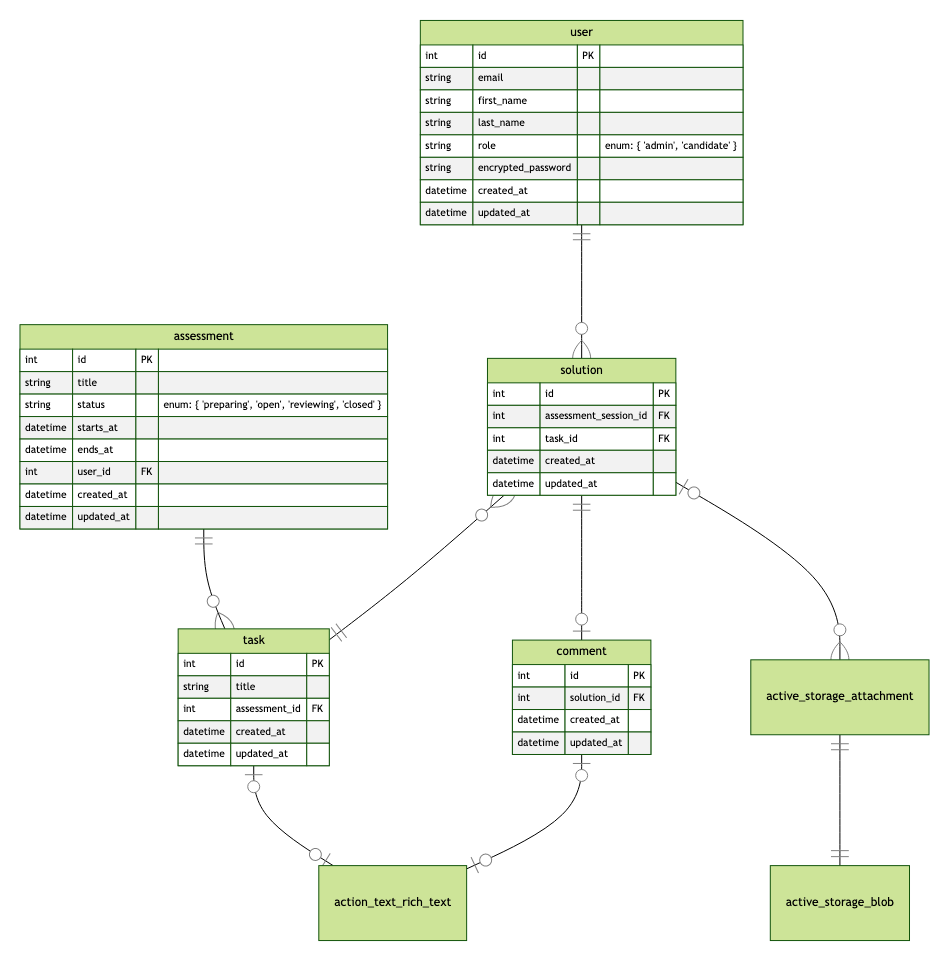
\includegraphics[height=15cm]{images/diagrams/entity-relation.png}
    \caption{\label{fig:erd} Entity-relationship Diagramm}
\end{figure}

\newpage

Sowohl der Zustand (State) von einem \emph{assessment} als auch die Benutzerrolle von einem \emph{user} wird in Form eines Enums abgebildet. Dabei ist zu beachten, dass es in der Praxis kein Database-Level Enum sein wird,
sondern der Wert in Form eines Strings in der Datenbank gespeichert werden soll. Der Constraint wird dann auf Application-Level durchgesetzt. Das ist ein ActiveRecord Standard und ermöglicht eine höhere Flexibilität und Erweiterbarkeit.
Ausserdem werden nicht alle Akteure aus \ref{tab:participants} in Form von Benutzerrollen in der \emph{user} Entität abgebildet, da die Zwei Akteure \enquote{Betreuer} und \enquote{Korrektor} in der Praxis die gleiche Person sein wird.

\subsection{Physisches Datenmodell (Generation)}

Das Ruby on Rails Framework bietet verschiedenste Command-Line Utilities, mit denen man sich relativ einfach gewisse
Grundstrukturen automatisiert generieren lassen Kann. Abgeleitet von \ref{fig:erd} können nun die ganzen Commands aufgestellt werden.
Werden diese ausgeführt, erstellen diese sowohl die dazugehörigen Model-Klassen, als auch alle notwendigen Datenbankmigrationen.

Die ganzen Assoziationen zwischen den Entitäten werden mit dem \emph{references} Typ schon bei der Generation abgebildet.
Bei dem \emph{rich\_text} Feldtyp handelt es sich um die bereits angesprochenen formatierten Textinhalte,
welche automatisch in eine andere Tabelle ausgelagert werden. Bei einem \emph{attachment} handelt es sich um einen anhängenden File-Upload.

\begin{figure}[H]
\begin{codebox}[]
\begin{minted}{shell}
bin/rails generate model Task title:string body:rich_text assessment:references
bin/rails generate model Assessment title:string status:string starts_at:datetime ends_at:datetime
bin/rails generate model Solution files:attachments task:references task:references user:references
bin/rails generate model Comment body:rich_text solution:references 
\end{minted}
\end{codebox}
\caption{\label{fig:generate-models}Commands für die automatisierte Generation von Model-Klassen}
\end{figure}

\newpage

\section{Zustandsdiagramm}

Während dem Lebenszyklus von einem \emph{assessment} durchläuft dieses mehrere Zustände. Diese ändern
sich durch Interaktionen gewisser Akteure mit dem System. Der Zustand verläuft relativ linear und es gibt kaum Sonderfälle.
Das Diagramm \ref{fig:state-diagram} versucht diesen Prozess zu veranschaulichen. Zwischen den Zuständen gibt es jeweils einen 
\emph{Trigger}, eine \emph{[Guard]} oder einen \emph{/Effect}.

\begin{figure}[H]
    \centering
    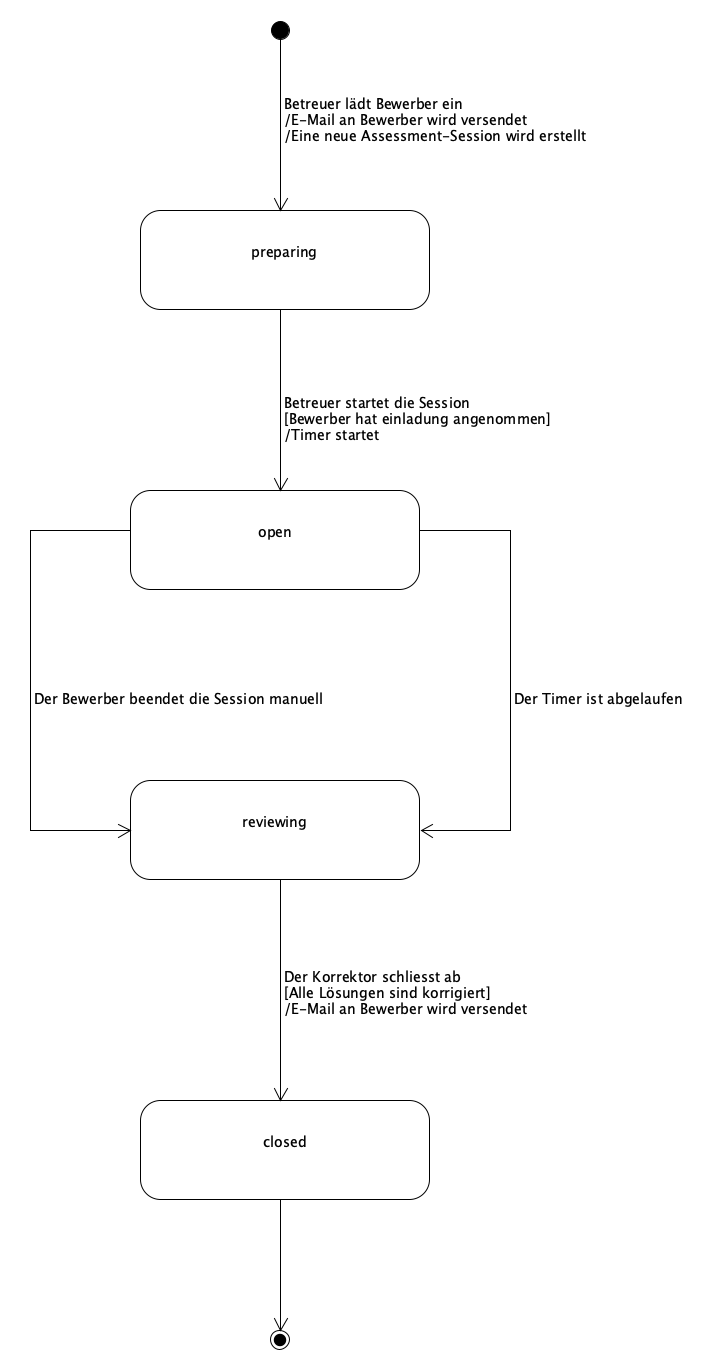
\includegraphics[height=17cm]{images/diagrams/state.png}
    \caption{\label{fig:state-diagram}UML Zustandsdiagramm eines Assessments}
\end{figure}

\newpage

\section{Mockups}

In diesem Abschnitt folgen grobe Entwürfe der verschiedenen Ansichten der Applikation. Diese sollen die Realisierung
erheblich vereinfachen und verschaffen nicht nur einen Überblick über das UI-Design, sondern . Kategorisiert wurden die Entwürfe nach den Akteuren \ref{tab:participants}

\subsection{Bewerber}
\begin{figure}[H]
    \centering
    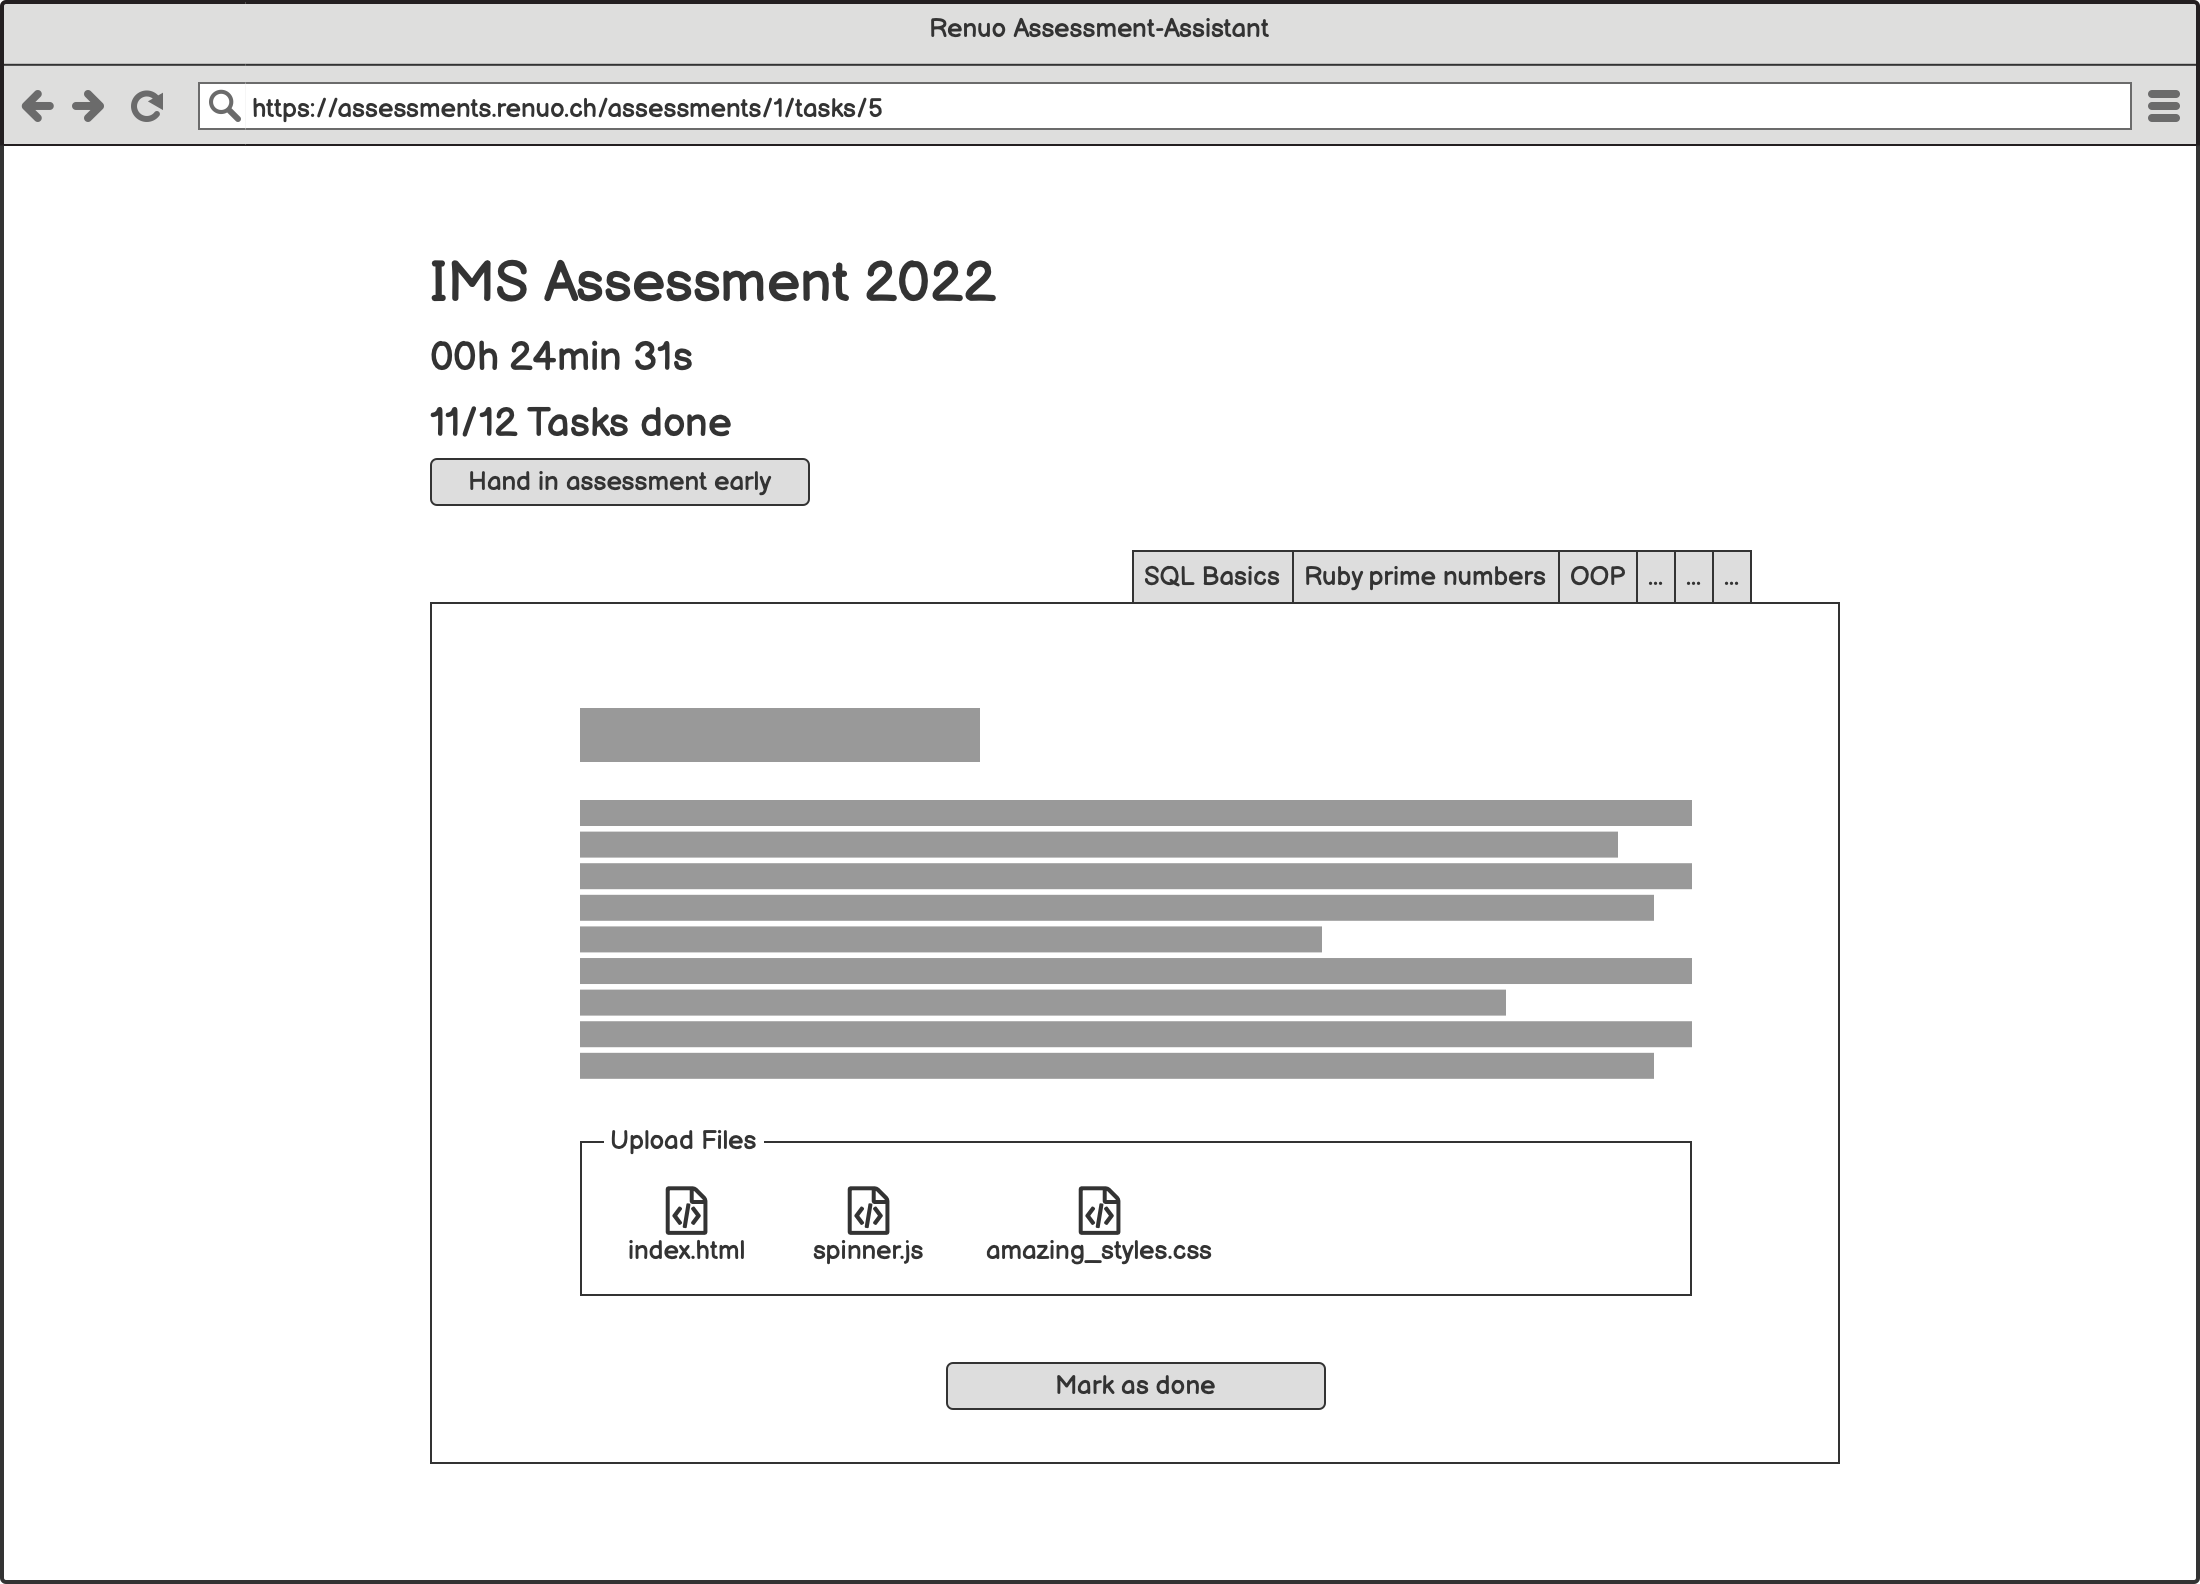
\includegraphics[width=12cm]{images/mockups/candidate-solve-assessment.png}
    \caption{\label{fig:mockup-candidate-solve-assessment}Entwurf für das Lösen eines Assessments}
\end{figure}

\subsection{Betreuer}
\begin{figure}[H]
    \centering
    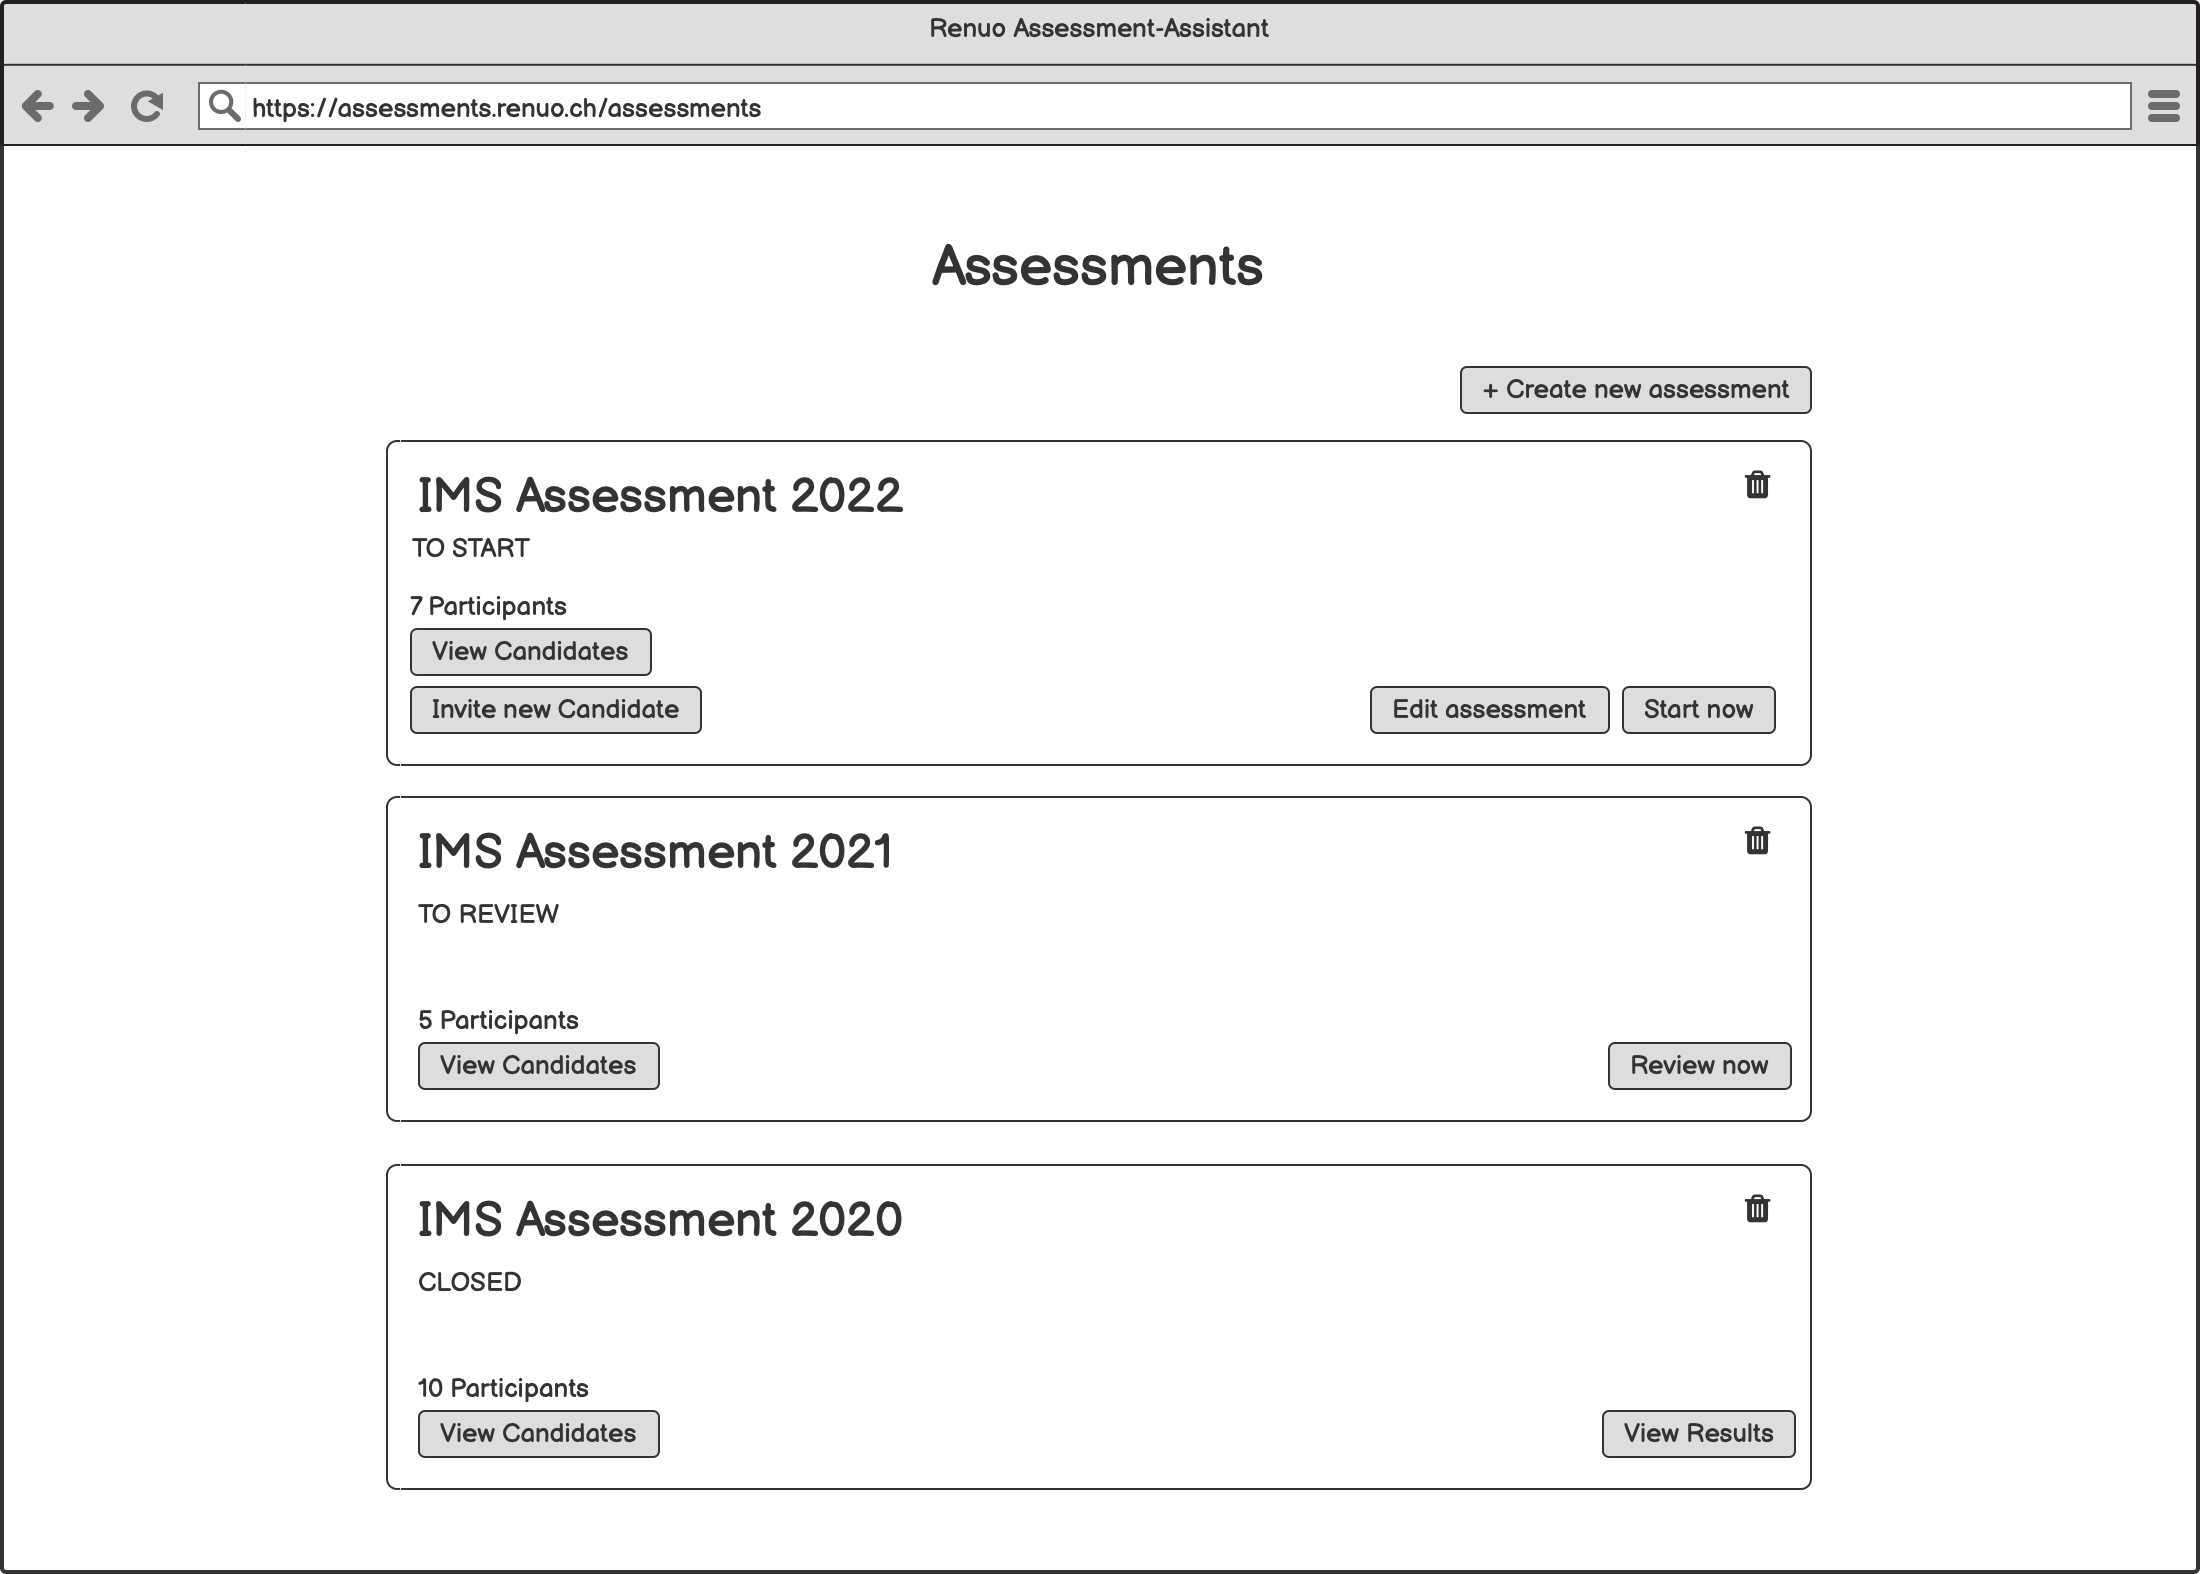
\includegraphics[width=12cm]{images/mockups/supervisor-list-assessments.png}
    \caption{\label{fig:mockup-supervisor-list-assessments}Entwurf für das Auflisten von Assessments}
\end{figure}
\begin{figure}[H]
    \centering
    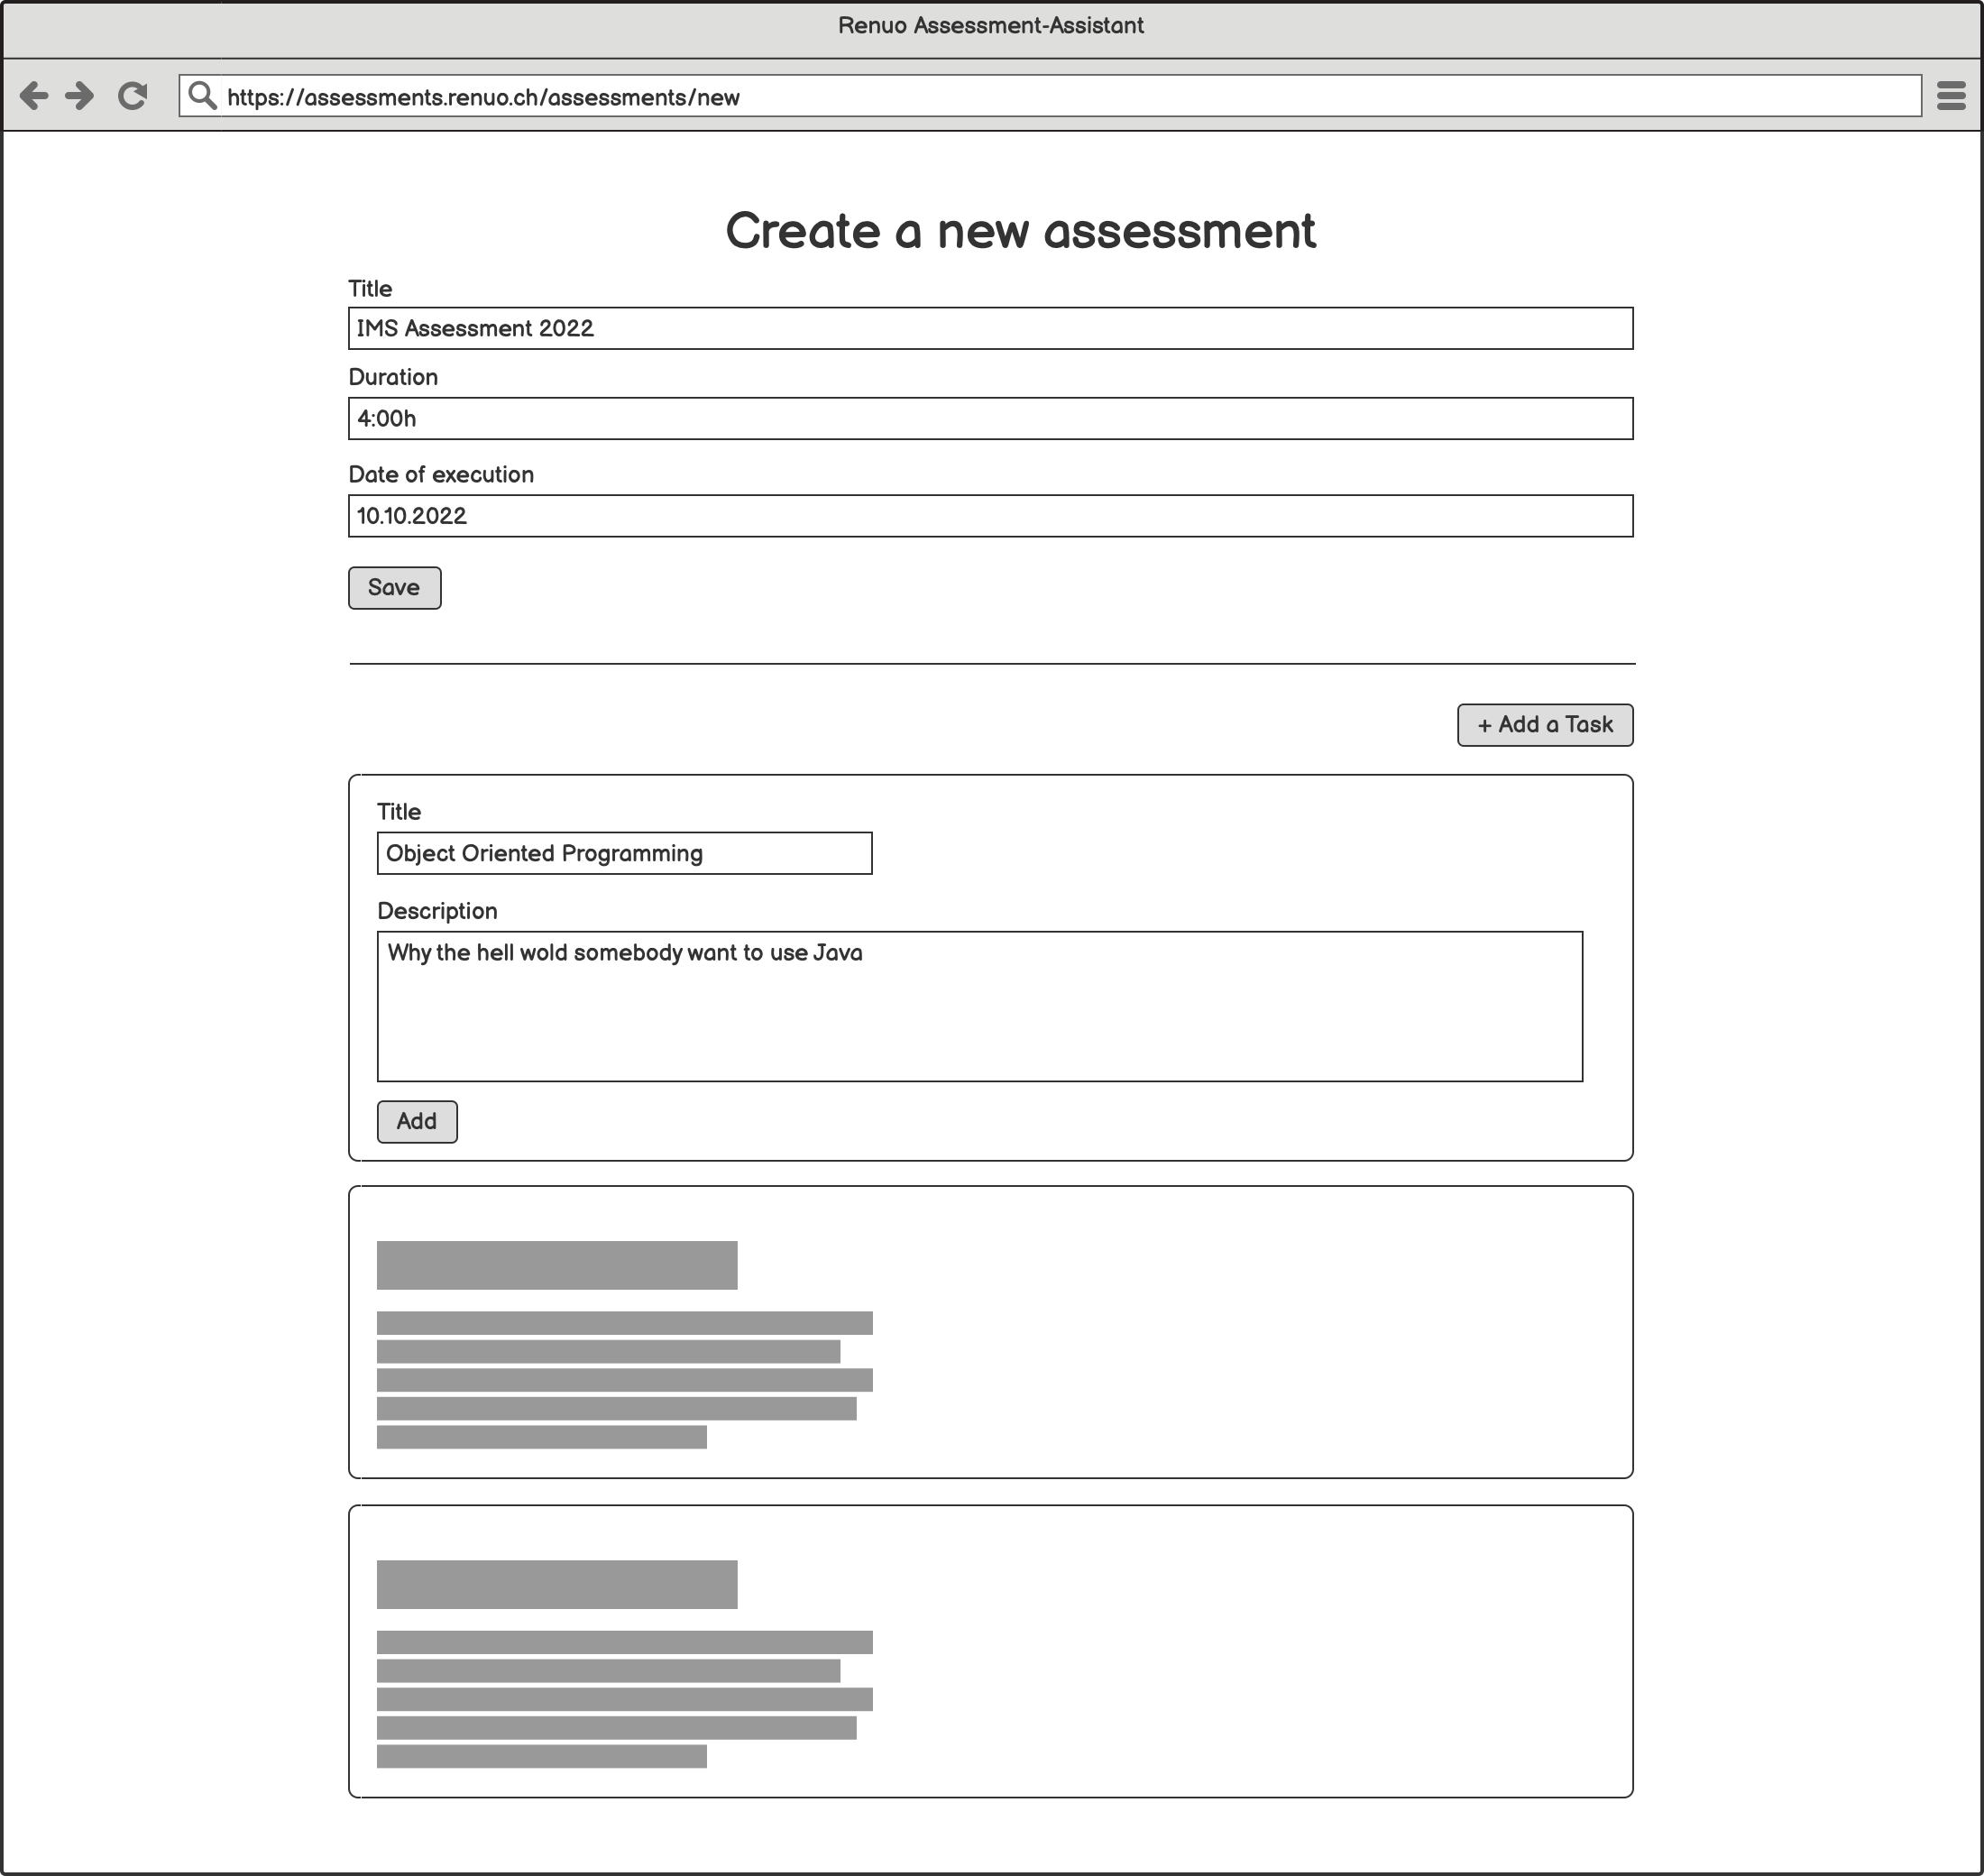
\includegraphics[width=12cm]{images/mockups/supervisor-create-assessment.png}
    \caption{\label{fig:mockup-supervisor-create-assessment}Entwurf für das Erstellen eines neuen Assessments}
\end{figure}

\subsection{Korrektor}
\begin{figure}[H]
    \centering
    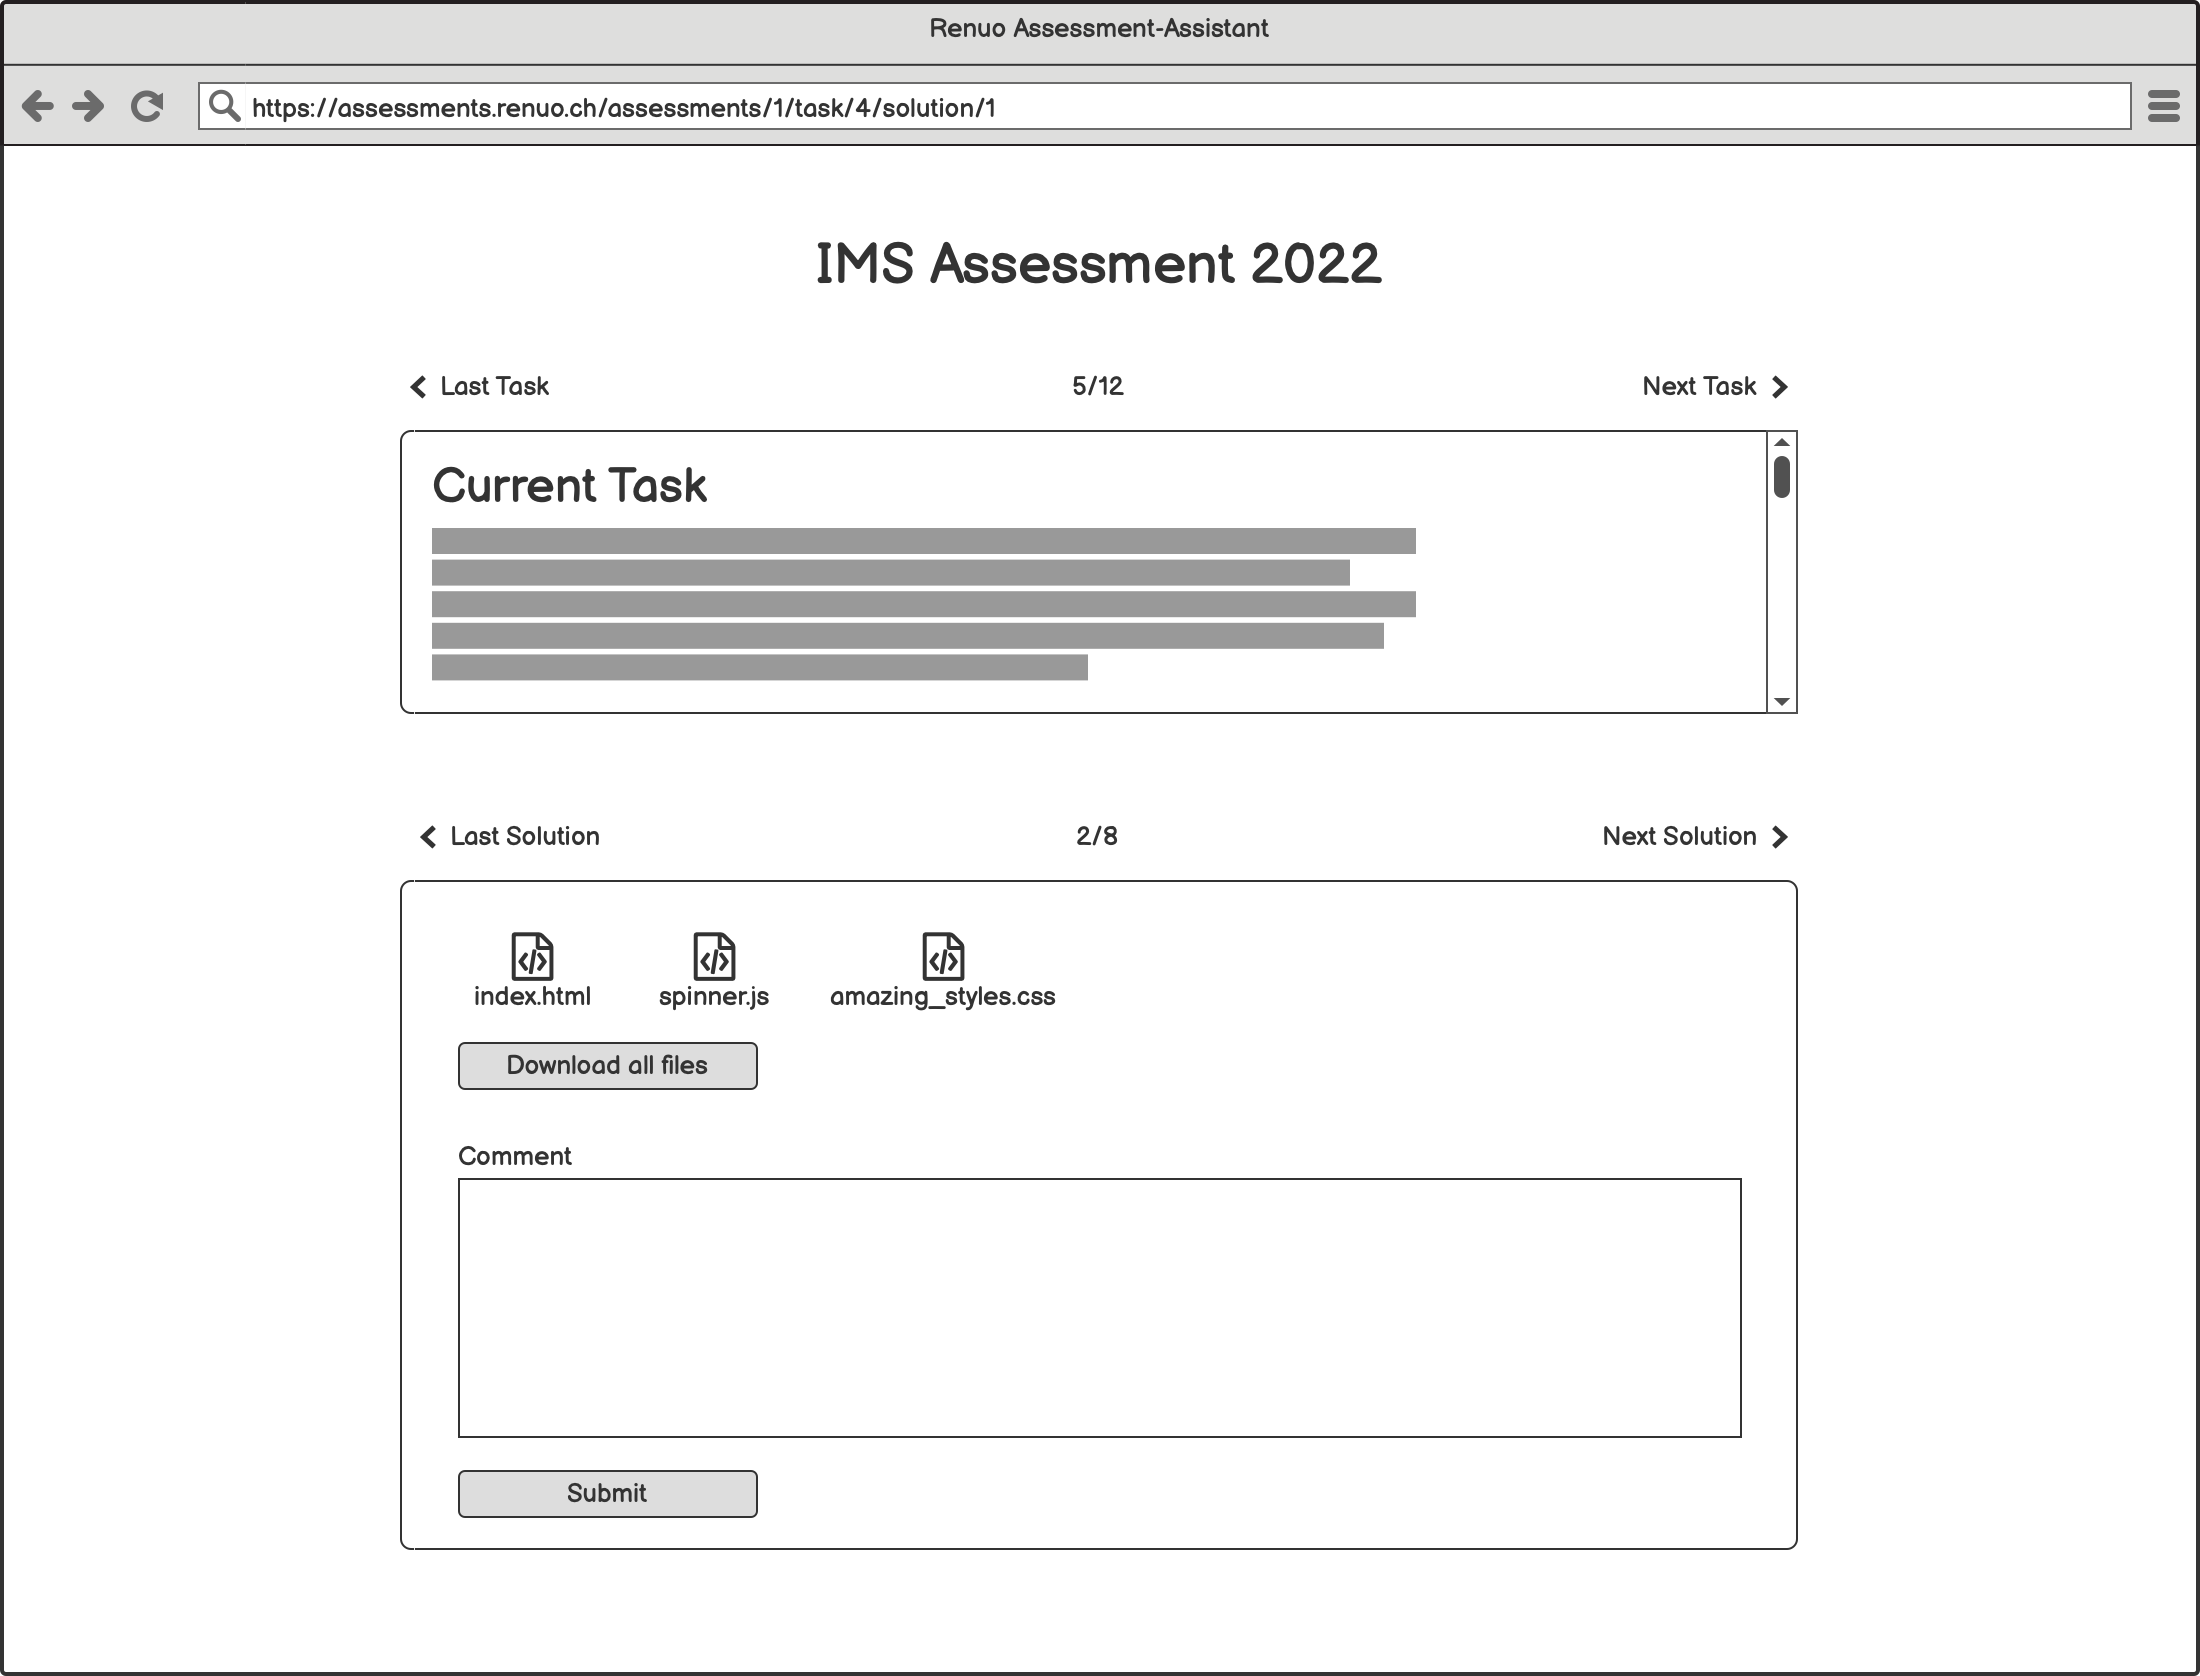
\includegraphics[width=12cm]{images/mockups/corrector-correct-assessment.png}
    \caption{\label{fig:mockup-solve-assessment}Entwurf für das Korrigieren eines Assessments}
\end{figure}
\begin{figure}[H]
    \centering
    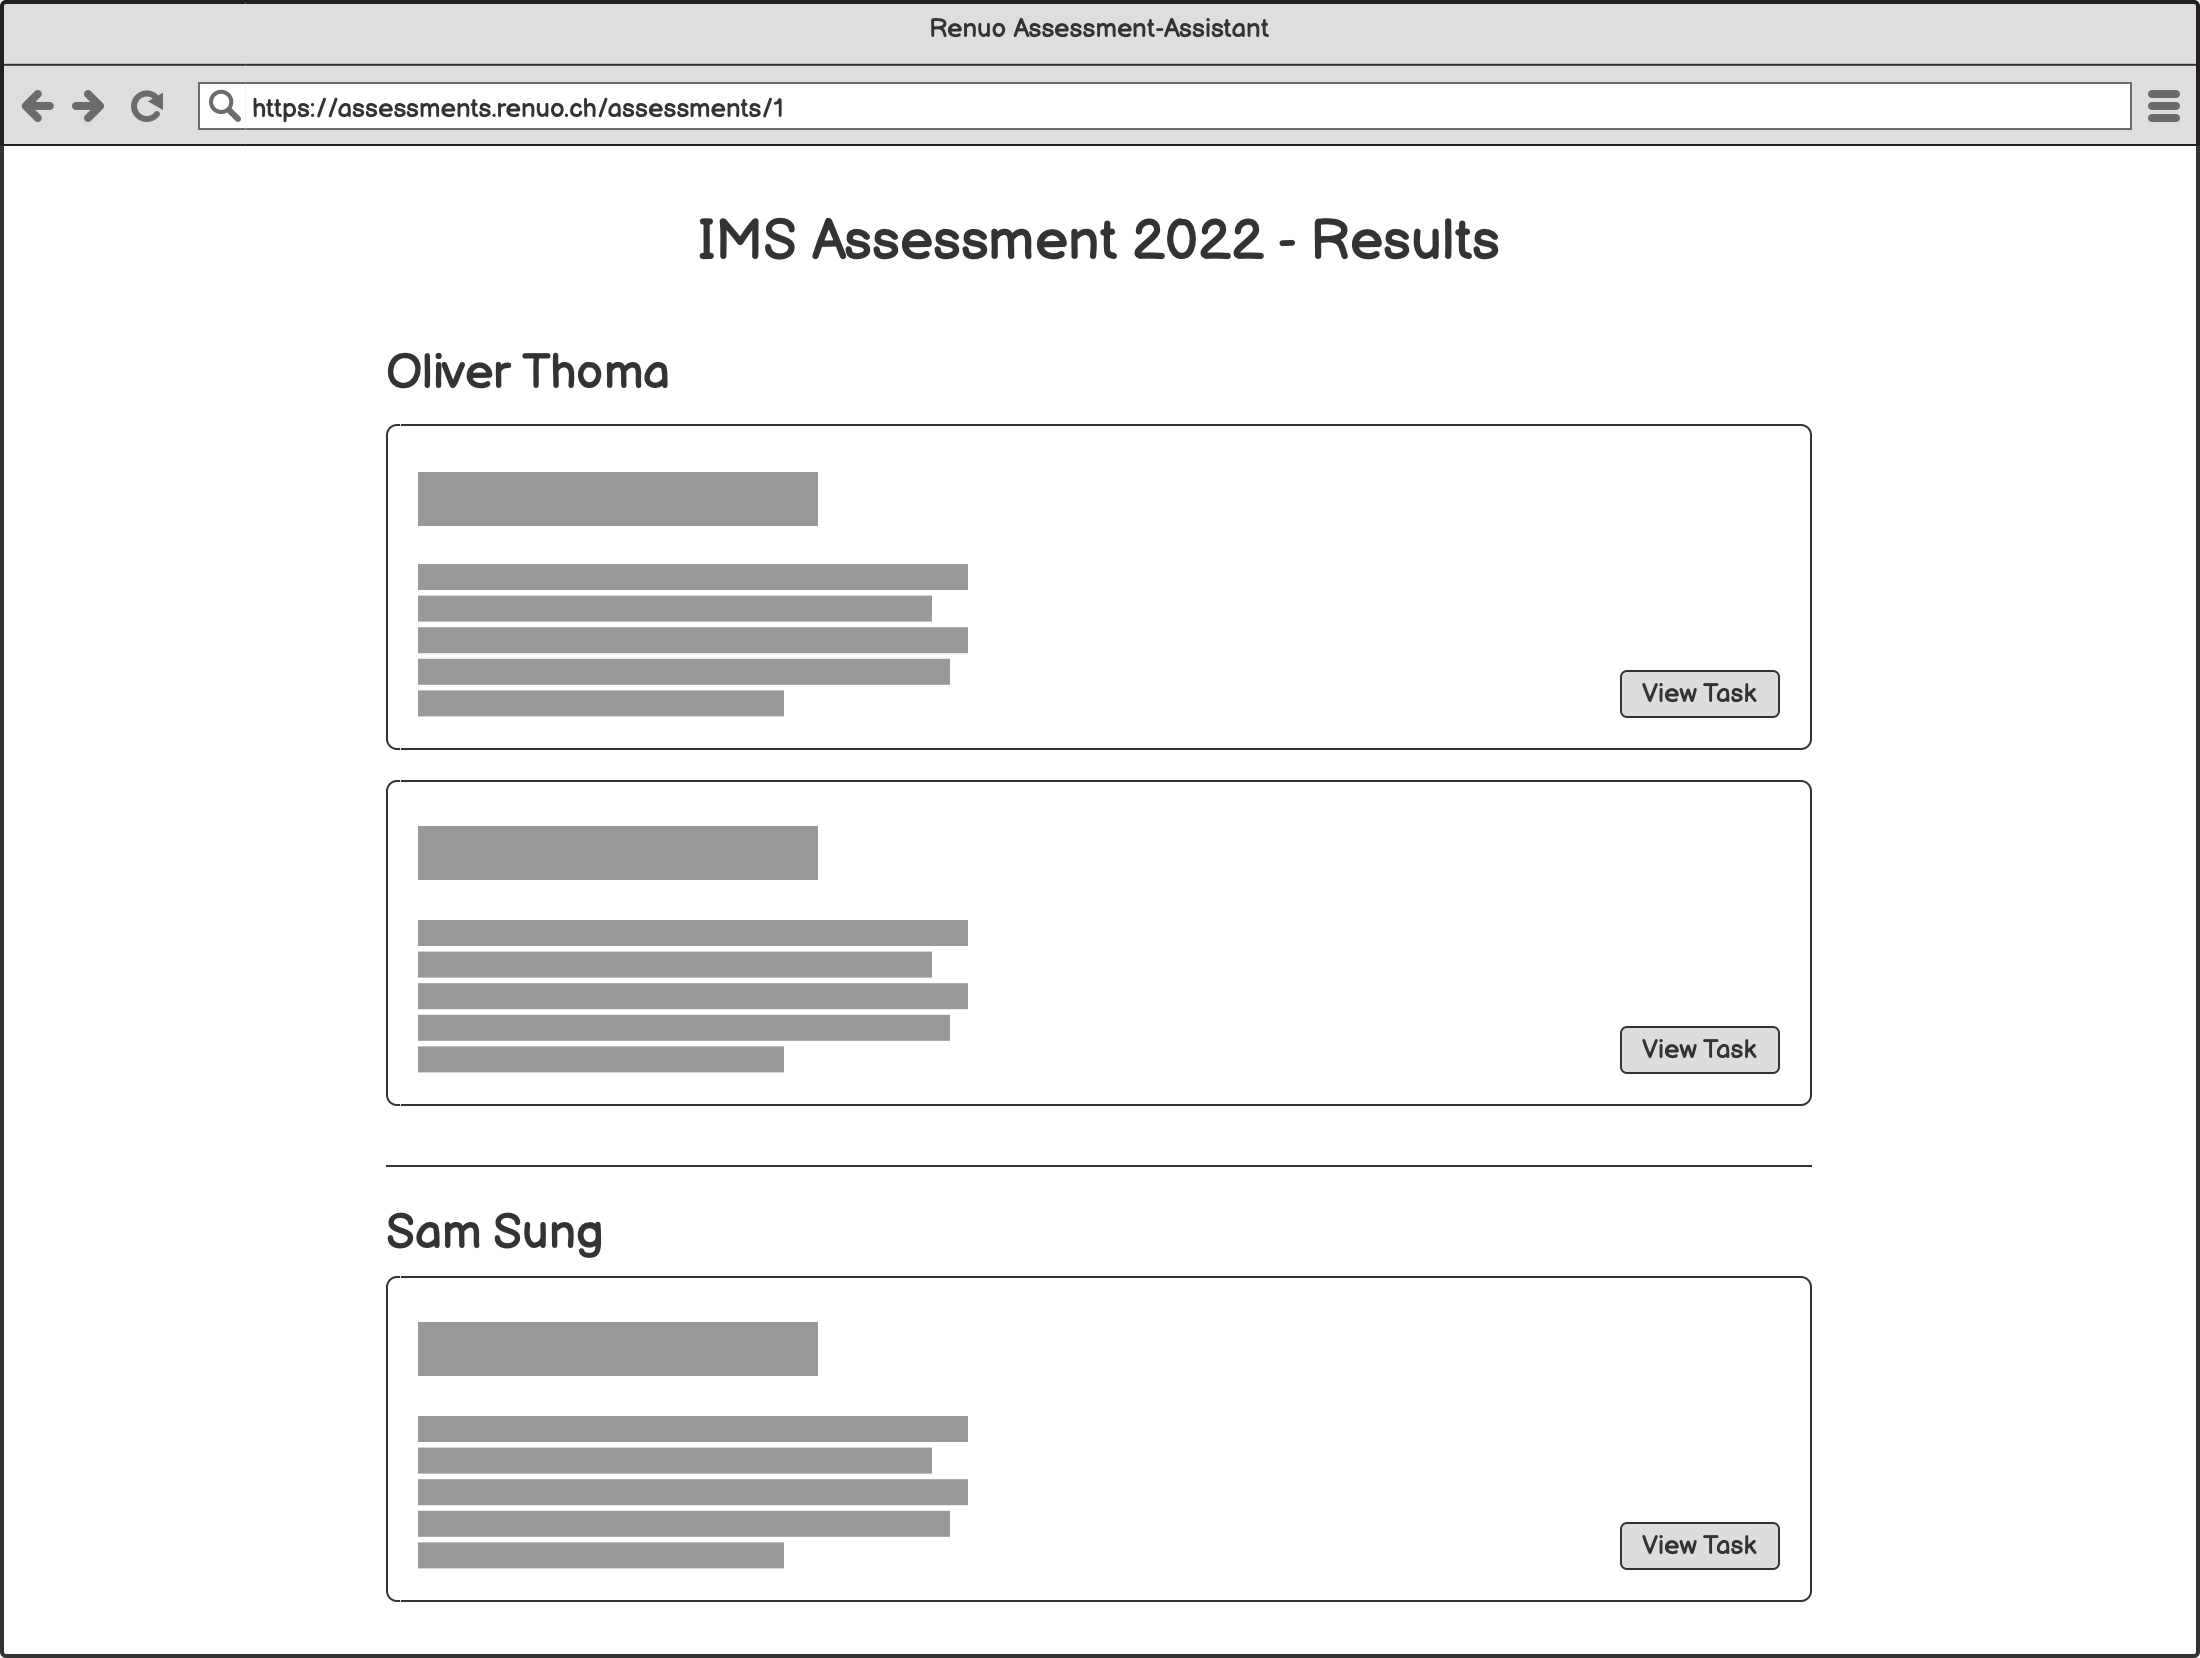
\includegraphics[width=12cm]{images/mockups/assessment-results.png}
    \caption{\label{fig:mockup-assessment-results}Entwurf für das Einsehen und Auflisten der Korrekturen}
\end{figure}

\newpage

\section{Testkonzept}

Das Testkonzept beschreibt, wie und mit welchen Werkzeugen das Resultat auf seine Richtigkeit kontrolliert wird.

\subsection{Testmethoden}

\subsubsection{Manuelle Tests}

\subsubsection{Automatisierte Tests}

\subsection{Testmittel}
